\section{Identifying Metamorphic Relations} \label{identifyingMR}
We identified five metamorphic properties for each dataset: rotation, shearing, shading, shifting the image along x-axis, and, shifting the image along y-axis. Each image in the testing dataset (digit, letter, and, fashion) was transformed using the five metamorphic properties. We used Keras image preprocessing functions to apply these transformations to the test data in each dataset to generate new data to measure robustness.

There are 10000 test images in the in the MNIST digit dataset. There are 10 class labels from 0 to 9, and each class label has 1000 instances. We applied the following metamorphic properties to each test image.
\subsection{Rotate}
Since we are dealing with image datasets, we hypothesize that small changes to the images by rotating them clock-wise or counter clock wise would not have drastic effect on the accuracy of model. To test our hypothesis we rotated the test data at each angle between [\ang{-50}, \ang{50}]. We also expect certain digits with symmetry (like 0) will be less afftected by these metamorphic properties.
 Each image in the test dataset was transformed using keras ImageDataGenerator method. 
The test images from each dataset is transformed The rotation transformation algorithm takes in an image and an angle in degrees as parameter and rotates the image with the given angle. For each angle in [\ang{-50}, \ang{50}] we transformed each image Each image (digit, letter, and, fashion) is rotated clockwise and counter clockwise between angles [\ang{-50}, \ang{50}]. 
    \begin{figure}[!htbp]
        \centering
        \begin{subfigure}[b]{.3\textwidth}
            \centering
            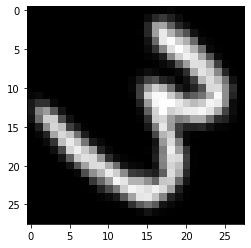
\includegraphics[width=\linewidth]{images/rotate1.png}
            \caption{Angle: \ang{-50}}
            \label{fig:Rotate-misclass0}
        \end{subfigure}%
        \begin{subfigure}[b]{.3\textwidth}
            \centering
            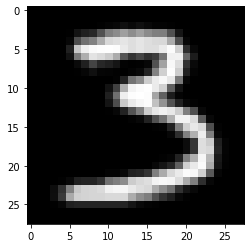
\includegraphics[width=\textwidth]{images/rotate2.png}
            \caption{Angle: \ang{0}}
            \label{fig:Rotate-misclass0}
        \end{subfigure}%
        \begin{subfigure}[b]{.3\textwidth}
            \centering
            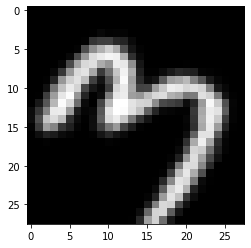
\includegraphics[width=\linewidth]{images/rotate3.png}
            \caption{Angle: \ang{50}}
            \label{fig:Rotate-misclass0}
        \end{subfigure}
        \caption{Rotation property applied to Digit 3.}
        \label{fig:Rotate-misclassifications}
    \end{figure}
    \FloatBarrier

\subsection{Shear} 
To shear the images we used image pre-processing library offered by Keras. The ImageDataGenerator class generates batches of tensor image data with real-time data augmentation. We used the ImageDataGenerator's $apply\_transform()$ method to apply a transformation to an image according to given parameters. The $apply\_transform()$ method takes in the image, transformation type, and, the amount of transformation to be applied as parameter. It then applies the transformation and returns a transformed version of the input in the same shape.
The transformation parameter we used here was $shear$ and the images were transformed between angle $[-50, 50]$.

    \begin{figure}[!htbp]
        \centering
        \begin{subfigure}[b]{.3\textwidth}
            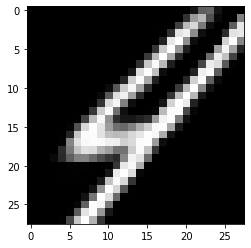
\includegraphics[width=\linewidth]{images/shear1.png}
            \caption{Angle: \ang{-50}}
            \label{fig:Rotate-misclass0}
        \end{subfigure}%
        \begin{subfigure}[b]{.3\textwidth}
            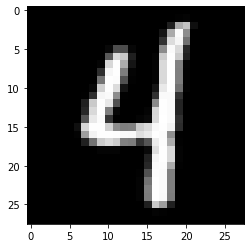
\includegraphics[width=\textwidth]{images/shear2.png}
            \caption{Angle: \ang{-50}}
            \label{fig:Rotate-misclass0}
        \end{subfigure}%
        \begin{subfigure}[b]{.3\textwidth}
            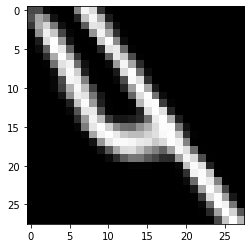
\includegraphics[width=\linewidth]{images/shear3.png}
            \caption{Angle: \ang{-50}}
            \label{fig:Rotate-misclass0}
        \end{subfigure}
        
        \caption{Shear property applied to Digit 4.}
        \label{fig:Rotate-misclassifications}
    \end{figure}
    \FloatBarrier
    
\subsection{Shading}
We represent the pixels of the MNIST images as floats between 0 and 1 where, 0 is white and 1 represents black. To apply the shading transformation we added values to the white pixels of the test data until they become black.
    \begin{figure}[htb!]
        \centering
        \begin{subfigure}[b]{.3\textwidth}
            \centering
            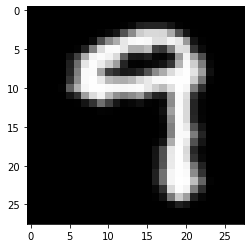
\includegraphics[width=\linewidth]{images/shade1.png}
            \caption{Value: 0}
            \label{fig:Rotate-misclass0}
        \end{subfigure}%
        \begin{subfigure}[b]{.3\textwidth}
            \centering
            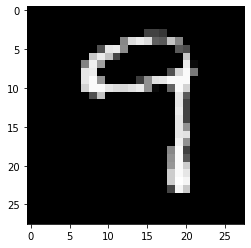
\includegraphics[width=\textwidth]{images/shade2.png}
            \caption{Value: 80}
            \label{fig:Rotate-misclass0}
        \end{subfigure}%
        \begin{subfigure}[b]{.3\textwidth}
            \centering
            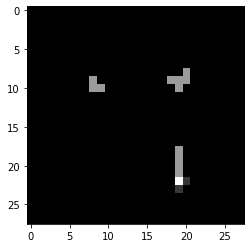
\includegraphics[width=\linewidth]{images/shade3.png}
            \caption{Value: 99}
            \label{fig:Rotate-misclass0}
        \end{subfigure}
        
        \caption{Shade property applied to Digit 9.}
        \label{fig:Rotate-misclassifications}
    \end{figure}
    \FloatBarrier
    
\subsection{Shifting in the X direction}
Since the images were 28 pixels wide, shifting the images by more than 28 pixels in either direction moved the images out of the frame completely. Thus, we transformed the test datasets by moving each image by pixels between 0 and 28 in both the X directions. We used ImageDataGenerator's $apply\_transform()$ function with $tx$ parameter to perform this transformation.
    \begin{figure}[htb!]
        \centering
        \begin{subfigure}[b]{.3\textwidth}
            \centering
            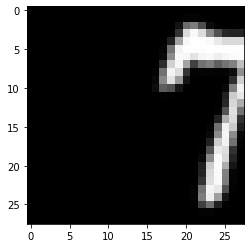
\includegraphics[width=\linewidth]{images/shiftx1.png}
            \caption{Value: 10}
            \label{fig:Rotate-misclass0}
        \end{subfigure}%
        \begin{subfigure}[b]{.3\textwidth}
            \centering
            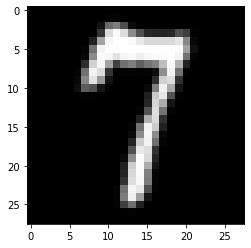
\includegraphics[width=\textwidth]{images/shiftx2.png}
            \caption{Value: 0}
            \label{fig:Rotate-misclass0}
        \end{subfigure}%
        \begin{subfigure}[b]{.3\textwidth}
            \centering
            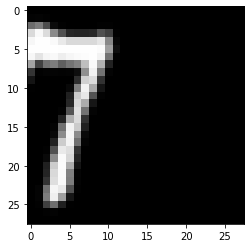
\includegraphics[width=\linewidth]{images/shiftx3.png}
            \caption{Value: -10}
            \label{fig:Rotate-misclass0}
        \end{subfigure}
        
        \caption{Shift X property applied to Digit 7.}
        \label{fig:Rotate-misclassifications}
    \end{figure}
    \FloatBarrier
    
\subsection{Shifting in the Y direction(ShiftY)}
The last metamorphic property we identified was shifting the images on Y axis. We used ImageDataGenerator's $apply\_transform()$ function with $ty$ parameter to transform the test data. Since the images are 28x28 pixels we shifted the images by each pixel between 0 and 28 pixels in both direction. 
    \begin{figure}[htb!]
        \centering
        \begin{subfigure}[b]{.3\textwidth}
            \centering
            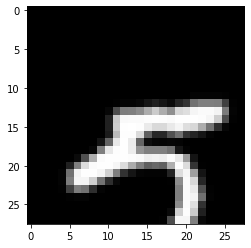
\includegraphics[width=\linewidth]{images/shifty1.png}
            \caption{Value: -10}
            \label{fig:Rotate-misclass0}
        \end{subfigure}%
        \begin{subfigure}[b]{.3\textwidth}
            \centering
            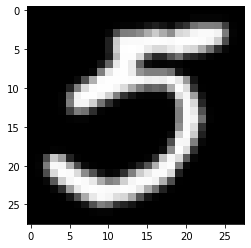
\includegraphics[width=\textwidth]{images/shifty2.png}
            \caption{Value: 0}
            \label{fig:Rotate-misclass0}
        \end{subfigure}%
        \begin{subfigure}[b]{.3\textwidth}
            \centering
            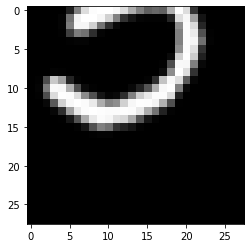
\includegraphics[width=\linewidth]{images/shifty3.png}
            \caption{Value: 10}
            \label{fig:Rotate-misclass0}
        \end{subfigure}
        
        \caption{Shift Y property applied to Digit 5.}
        \label{fig:Rotate-misclassifications}
    \end{figure}
    \FloatBarrier

After generating all the transformed versions of the datasets they were saved to be used as follow-up test cases for our machine-learning algorithms.